\begin{appendices}
    \chapter{MONKS' learning curves} % (fold)
    \label{cha:monks_learning_curves}
        Here we present the \textit{learning curves} for the three MONKS datasets. We have sampled these curves
        during the final tests on each dataset by plotting one of the 10 trails we used for building the
        statistics we presented in section \ref{sec:monks}, hence each plot presents a possible learning curve
        for the best hyperparameters' selection for each dataset.


        \section{Stochastic Gradient Descent} % (fold)
        \label{sec:stochastic_gradient_descent}
        % section stochastic_gradient_descent (end)

            \begin{figure}[H]
                \centering
                \begin{subfigure}{0.60\textwidth}
                    \resizebox{\textwidth}{!}{
                        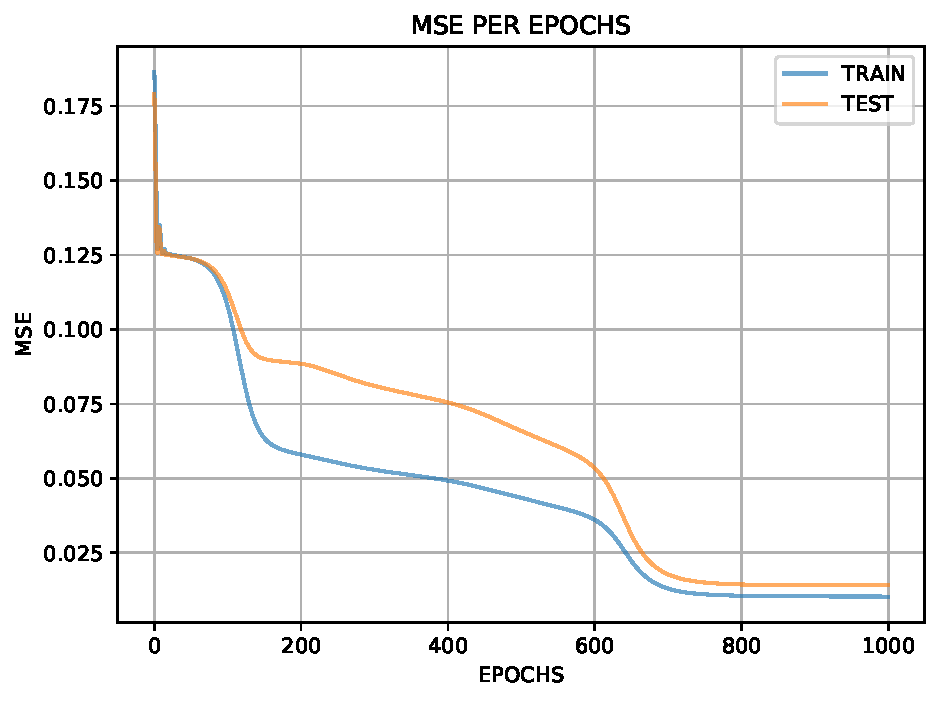
\includegraphics{img/SGD/sgd_mse_test_monks_1.pdf}
                    }
                    \caption{}
                    \label{fig:monks_1_MSE_SGD}
                \end{subfigure}
                \begin{subfigure}{0.60\textwidth}
                    \resizebox{\textwidth}{!}{
                        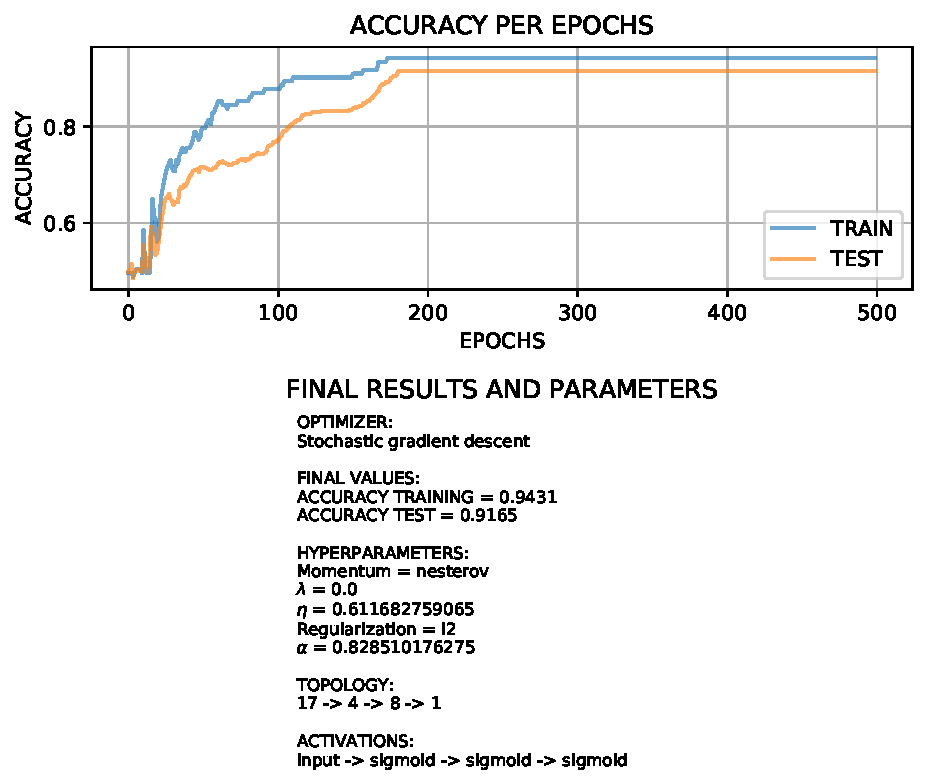
\includegraphics{img/SGD/sgd_accuracy_test_monks_1.pdf}
                    }
                    \caption{}
                    \label{fig:monks_1_ACC_SGD}
                \end{subfigure}
                \caption{Example of a final learning curve on MONKS 1.}
                \label{fig:monks_1_SGD}
            \end{figure}

            \begin{figure}[H]
                \centering
                \begin{subfigure}{0.60\textwidth}
                    \resizebox{\textwidth}{!}{
                        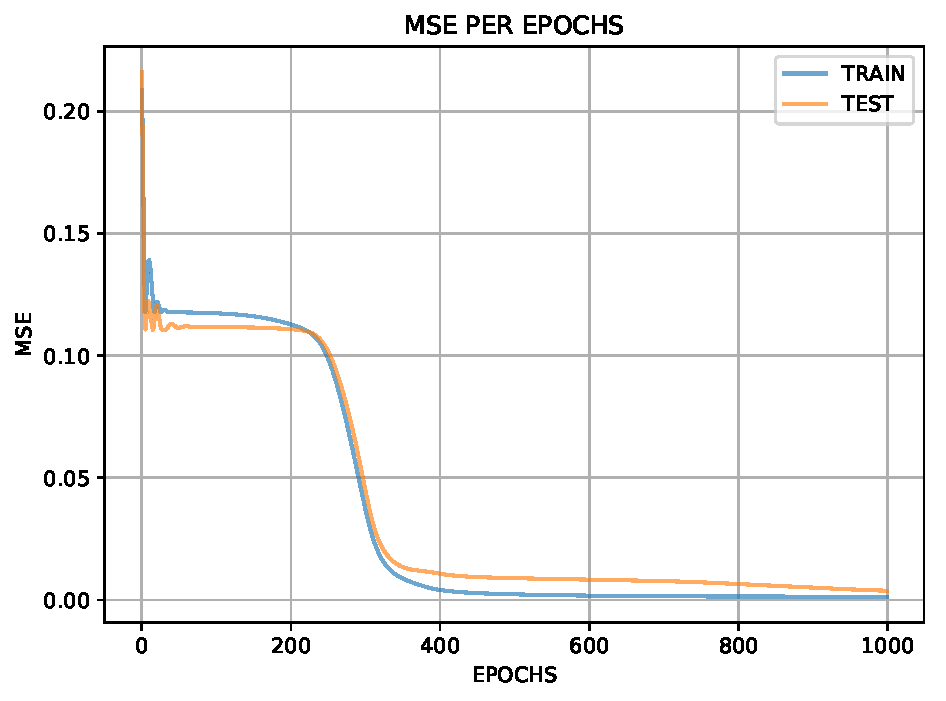
\includegraphics{img/SGD/sgd_mse_test_monks_2.pdf}
                    }
                    \caption{}
                    \label{fig:monks_2_MSE_SGD}
                \end{subfigure}
                \begin{subfigure}{0.60\textwidth}
                    \resizebox{\textwidth}{!}{
                        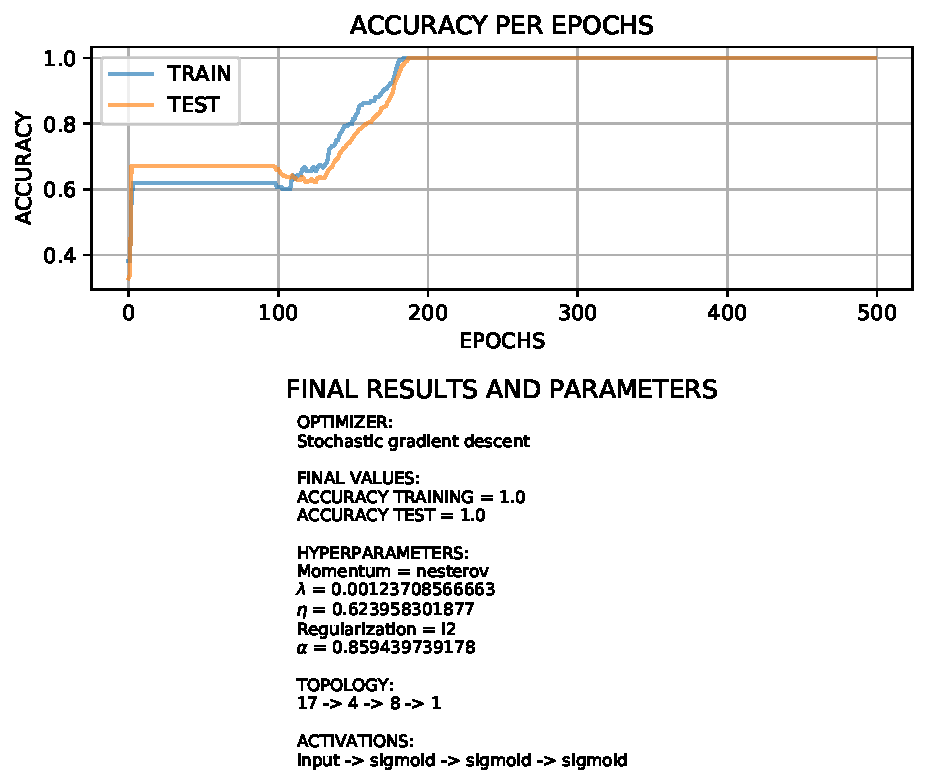
\includegraphics{img/SGD/sgd_accuracy_test_monks_2.pdf}
                    }
                    \caption{}
                    \label{fig:monks_2_ACC_SGD}
                \end{subfigure}
                \caption{Example of a final learning curve on MONKS 2.}
                \label{fig:monks_2_SGD}
            \end{figure}

            \begin{figure}[H]
                \centering
                \begin{subfigure}{0.60\textwidth}
                    \resizebox{\textwidth}{!}{
                        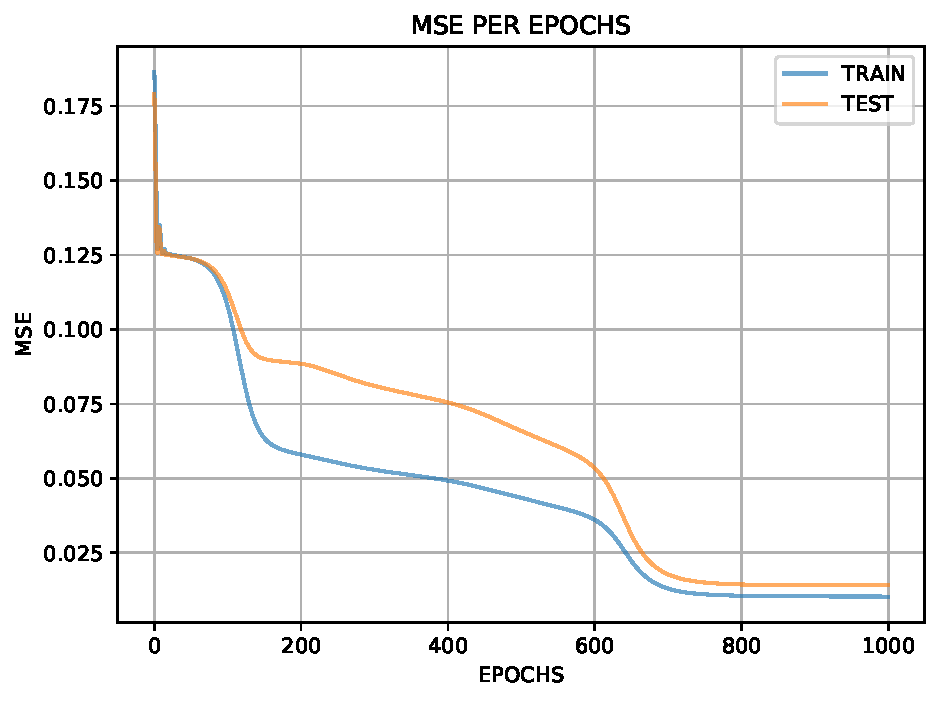
\includegraphics{img/SGD/sgd_mse_test_monks_1.pdf}
                    }
                    \caption{}
                    \label{fig:monks_3_MSE_SGD}
                \end{subfigure}
                \begin{subfigure}{0.60\textwidth}
                    \resizebox{\textwidth}{!}{
                        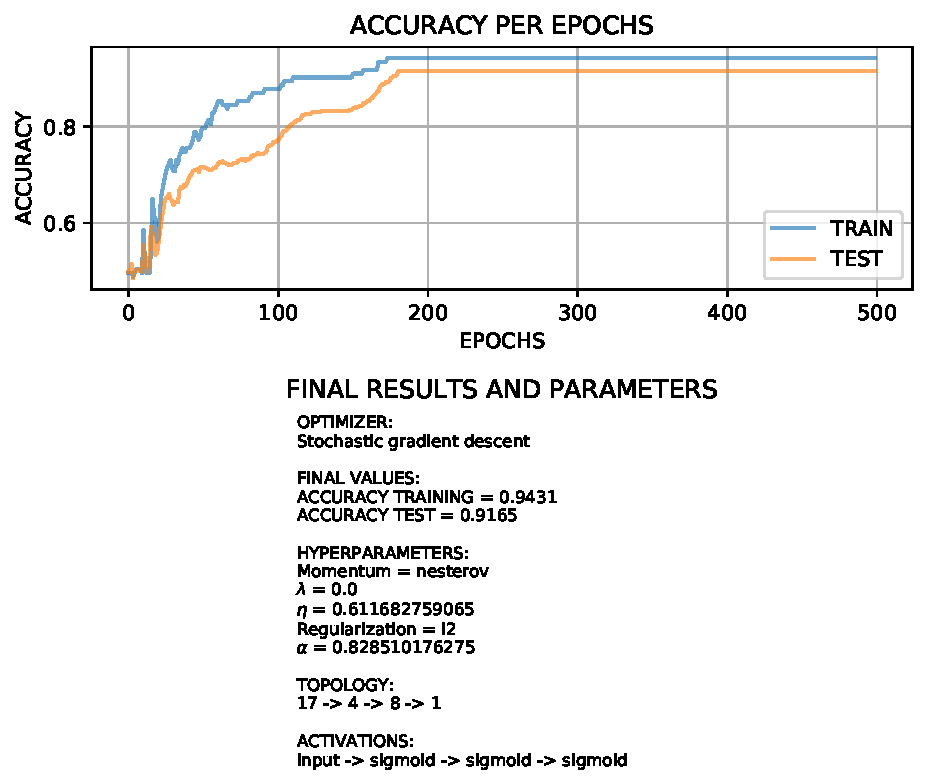
\includegraphics{img/SGD/sgd_accuracy_test_monks_1.pdf}
                    }
                    \caption{}
                    \label{fig:monks_3_ACC_SGD}
                \end{subfigure}
                \caption{Example of a final learning curve on MONKS 3.}
                \label{fig:monks_3_SGD}
            \end{figure}


        \section{Conjugate Gradient Methods} % (fold)
        \label{sec:conjugate_gradient_methods}

            \subsection{$MHS^+$} % (fold)
            \label{sub:mhs}

                \begin{figure}[H]
                    \centering
                    \begin{subfigure}{0.60\textwidth}
                        \resizebox{\textwidth}{!}{
                            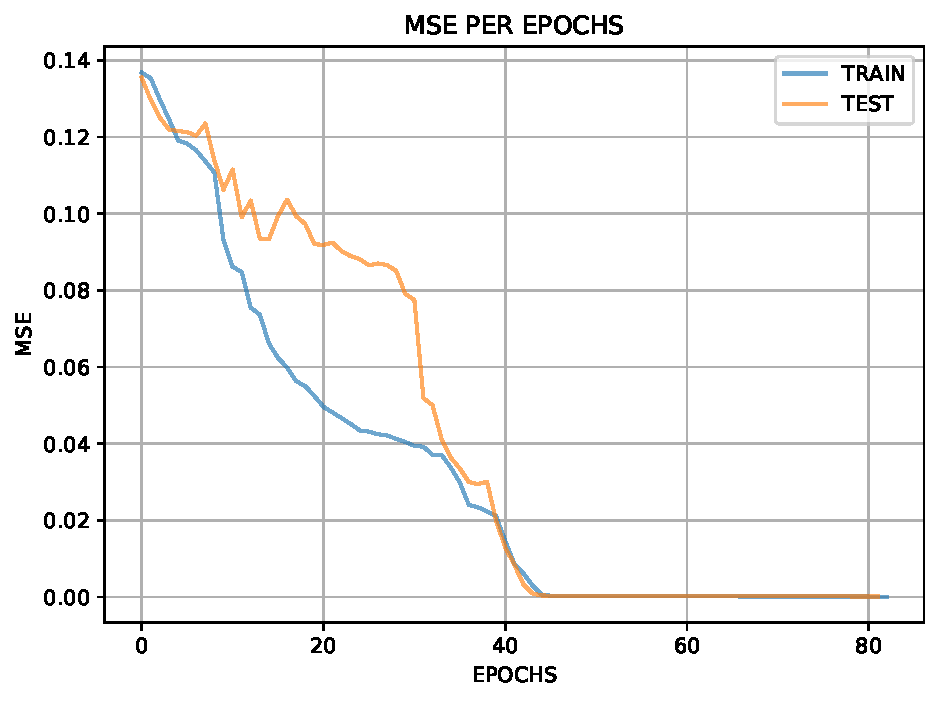
\includegraphics{img/CGD/MHS/cgd_mse_test_mhs_monks_1.pdf}
                        }
                        \caption{}
                        \label{fig:monks_1_MSE_CGD_MHS}
                    \end{subfigure}
                    \begin{subfigure}{0.60\textwidth}
                        \resizebox{\textwidth}{!}{
                            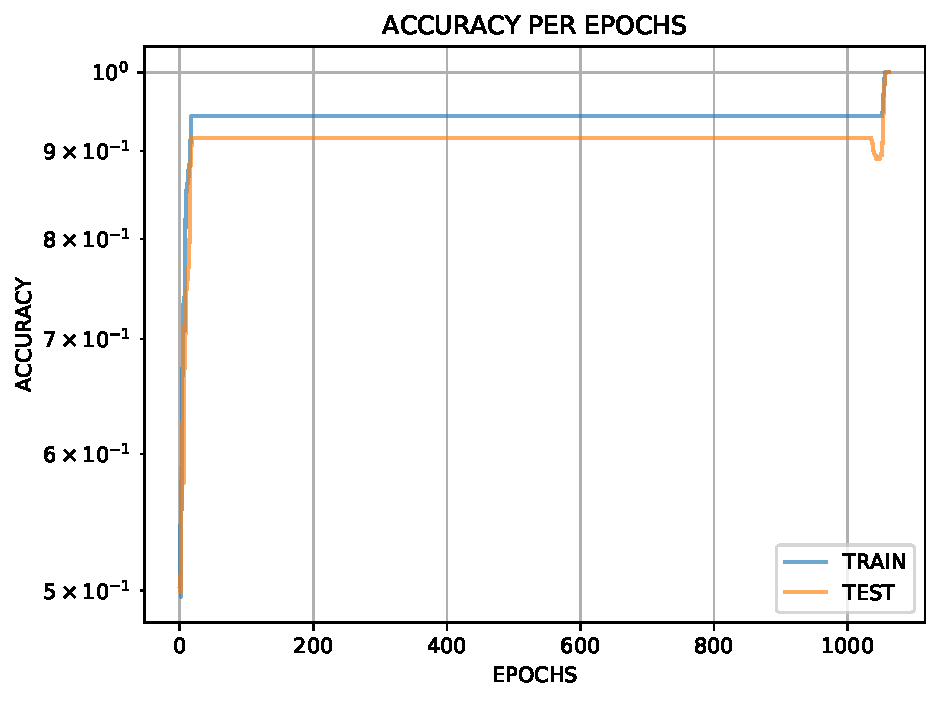
\includegraphics{img/CGD/MHS/cgd_accuracy_test_mhs_monks_1.pdf}
                        }
                        \caption{}
                        \label{fig:monks_1_ACC_CGD_MHS}
                    \end{subfigure}
                    \caption{Example of a final learning curve on MONKS 1.}
                    \label{fig:monks_1_CGD_MHS}
                \end{figure}

                \begin{figure}[H]
                    \centering
                    \begin{subfigure}{0.60\textwidth}
                        \resizebox{\textwidth}{!}{
                            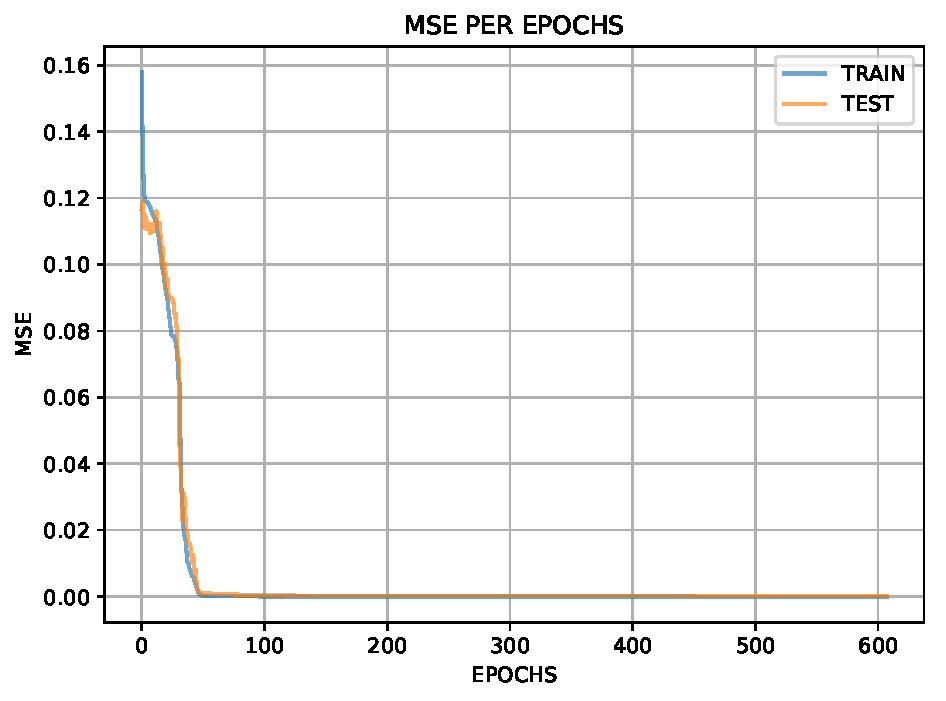
\includegraphics{img/CGD/MHS/cgd_mse_test_mhs_monks_2.pdf}
                        }
                        \caption{}
                        \label{fig:monks_2_MSE_CGD_MHS}
                    \end{subfigure}
                    \begin{subfigure}{0.60\textwidth}
                        \resizebox{\textwidth}{!}{
                            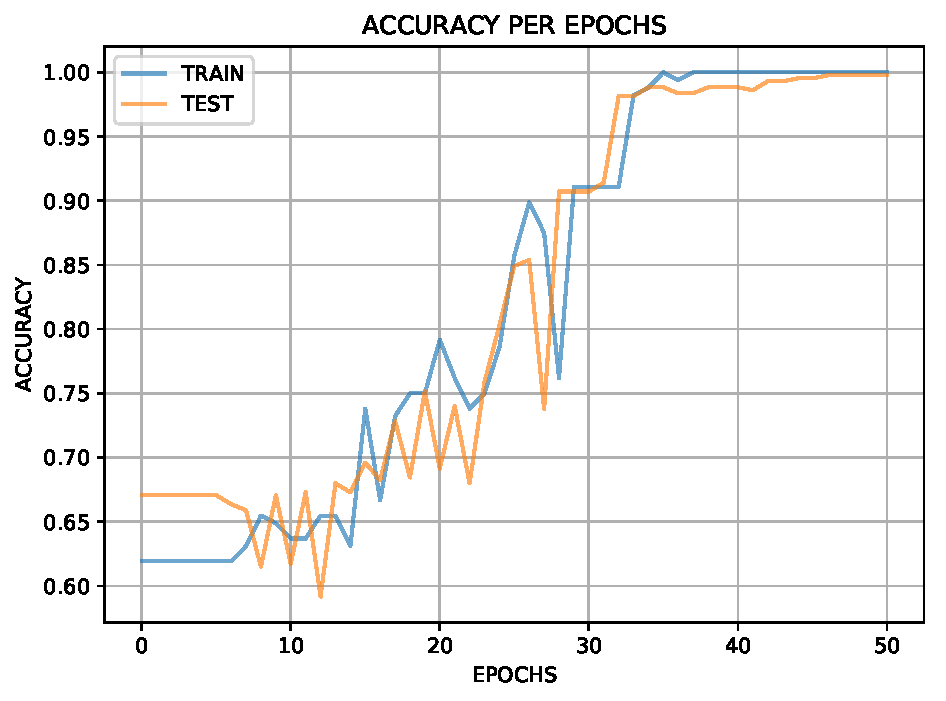
\includegraphics{img/CGD/MHS/cgd_accuracy_test_mhs_monks_2.pdf}
                        }
                        \caption{}
                        \label{fig:monks_2_ACC_CGD_MHS}
                    \end{subfigure}
                    \caption{Example of a final learning curve on MONKS 2.}
                    \label{fig:monks_2_CGD_MHS}
                \end{figure}

                \begin{figure}[H]
                    \centering
                    \begin{subfigure}{0.60\textwidth}
                        \resizebox{\textwidth}{!}{
                            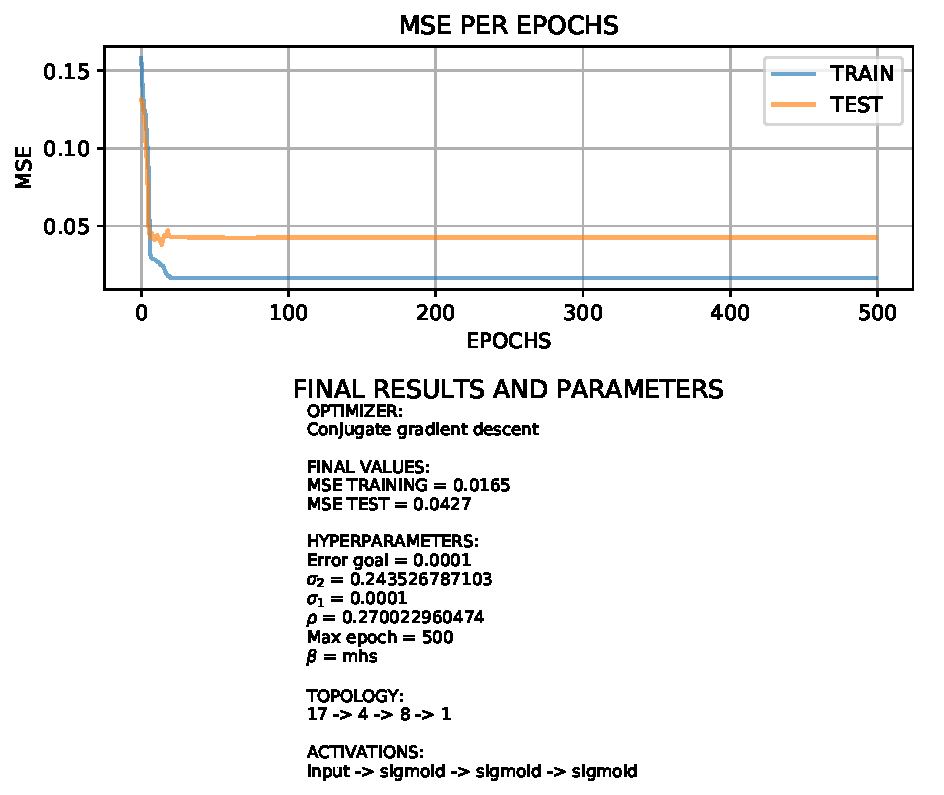
\includegraphics{img/CGD/MHS/cgd_mse_test_mhs_monks_3.pdf}
                        }
                        \caption{}
                        \label{fig:monks_3_MSE_CGD_MHS}
                    \end{subfigure}
                    \begin{subfigure}{0.60\textwidth}
                        \resizebox{\textwidth}{!}{
                            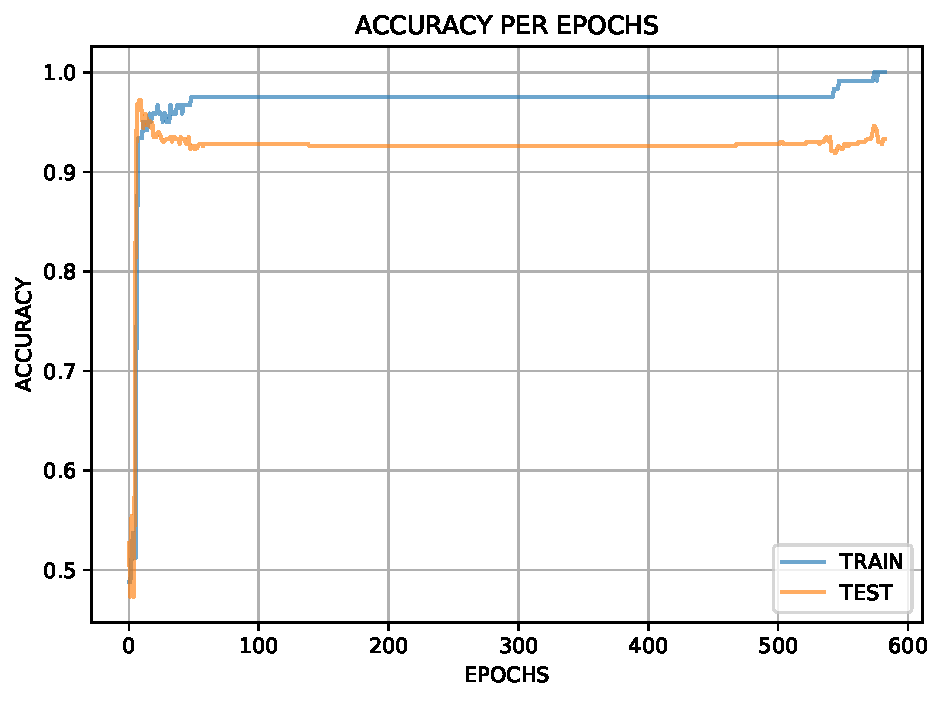
\includegraphics{img/CGD/MHS/cgd_accuracy_test_mhs_monks_3.pdf}
                        }
                        \caption{}
                        \label{fig:monks_3_ACC_CGD_MHS}
                    \end{subfigure}
                    \caption{Example of a final learning curve on MONKS 3.}
                    \label{fig:monks_3_CGD_MHS}
                \end{figure}

            % subsection mhs (end)

            \subsection{$HS^+$} % (fold)
            \label{sub:hs}

                \begin{figure}[H]
                    \centering
                    \begin{subfigure}{0.60\textwidth}
                        \resizebox{\textwidth}{!}{
                            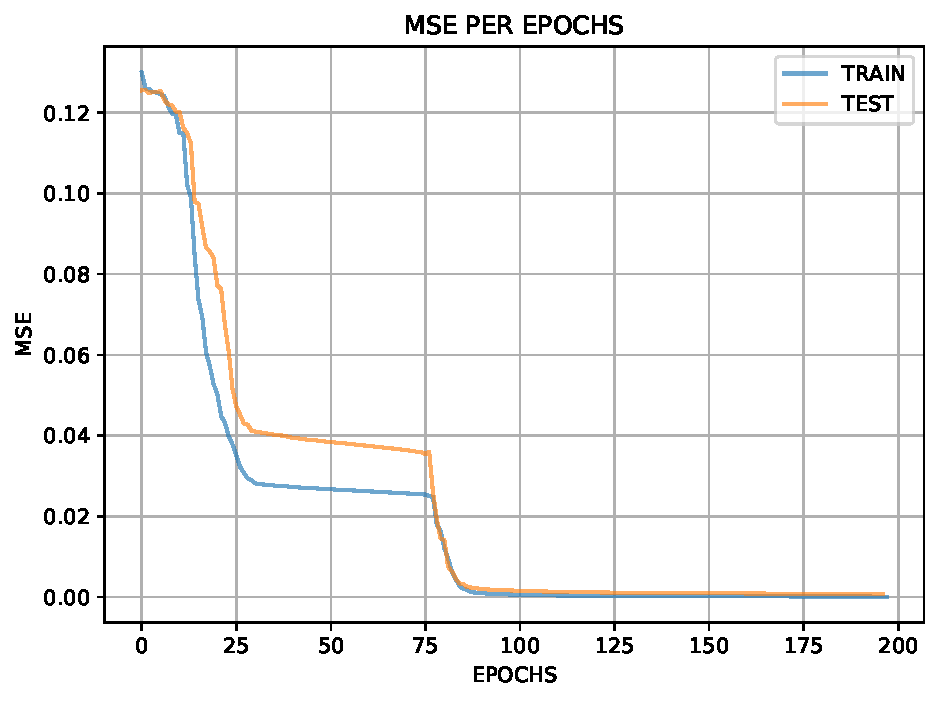
\includegraphics{img/CGD/HS/cgd_mse_test_hs_monks_1.pdf}
                        }
                        \caption{}
                        \label{fig:monks_1_MSE_CGD_HS}
                    \end{subfigure}
                    \begin{subfigure}{0.60\textwidth}
                        \resizebox{\textwidth}{!}{
                            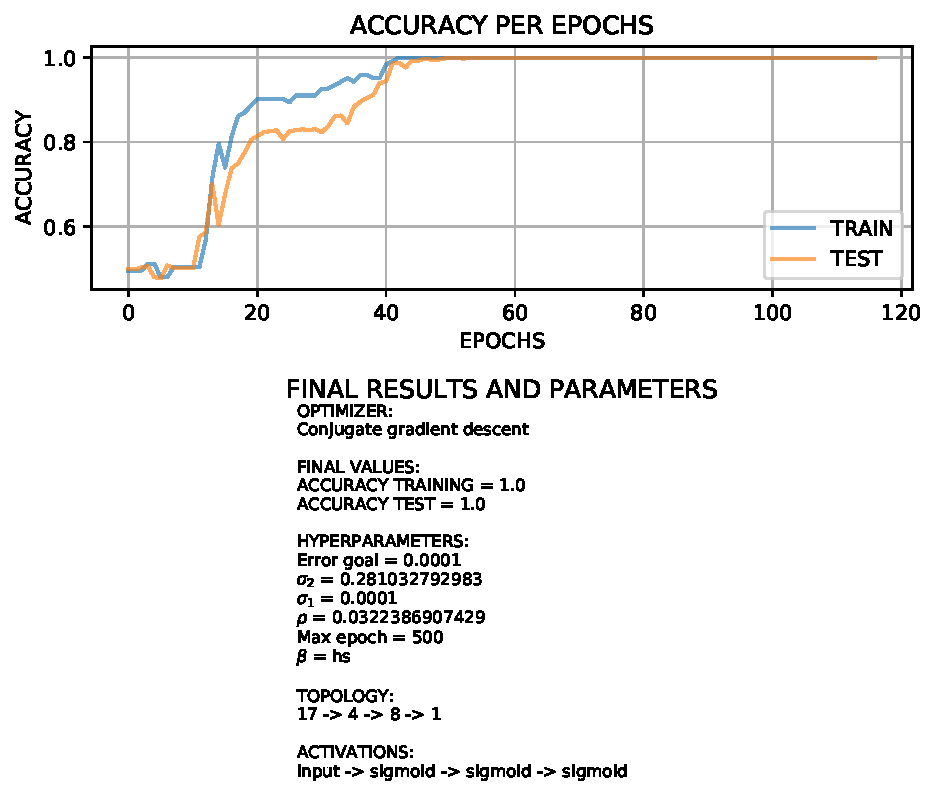
\includegraphics{img/CGD/HS/cgd_accuracy_test_hs_monks_1.pdf}
                        }
                        \caption{}
                        \label{fig:monks_1_ACC_CGD_HS}
                    \end{subfigure}
                    \caption{Example of a final learning curve on MONKS 1.}
                    \label{fig:monks_1_CGD_HS}
                \end{figure}

                \begin{figure}[H]
                    \centering
                    \begin{subfigure}{0.60\textwidth}
                        \resizebox{\textwidth}{!}{
                            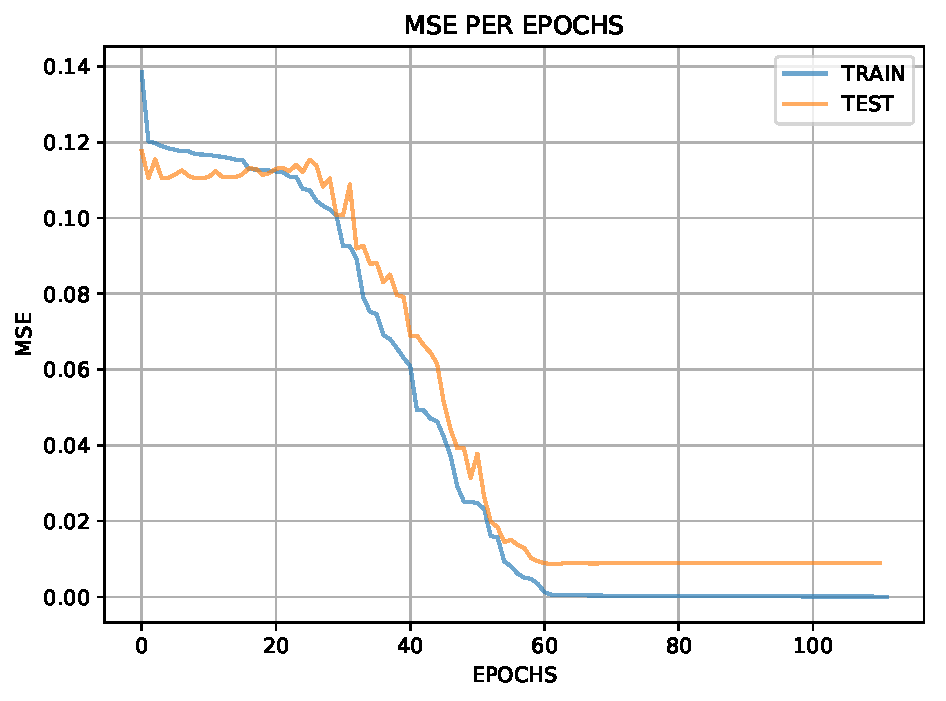
\includegraphics{img/CGD/HS/cgd_mse_test_hs_monks_2.pdf}
                        }
                        \caption{}
                        \label{fig:monks_2_MSE_CGD_HS}
                    \end{subfigure}
                    \begin{subfigure}{0.60\textwidth}
                        \resizebox{\textwidth}{!}{
                            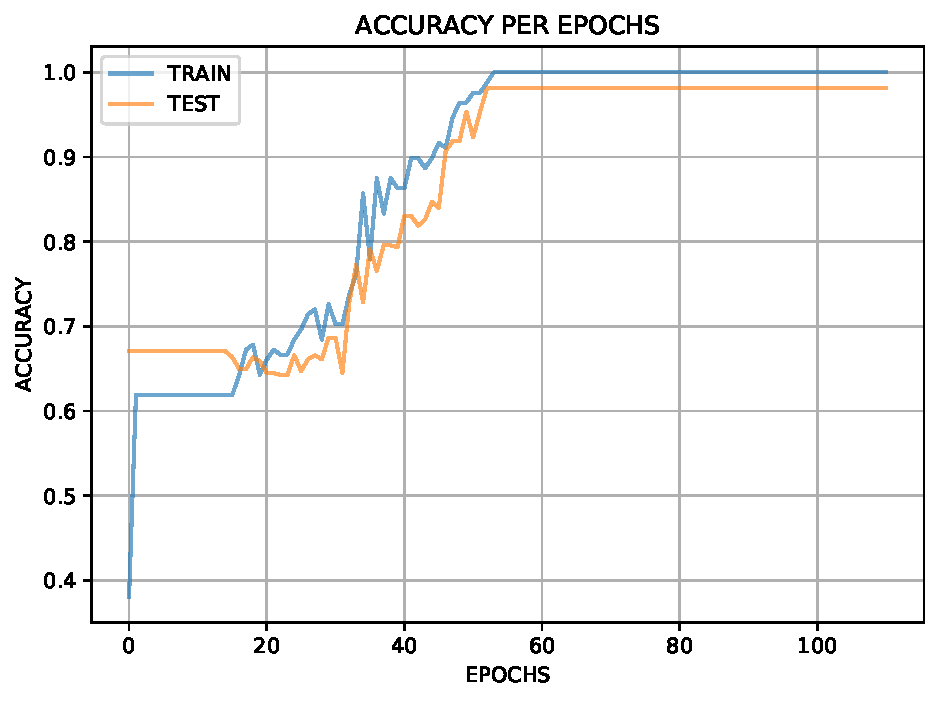
\includegraphics{img/CGD/HS/cgd_accuracy_test_hs_monks_2.pdf}
                        }
                        \caption{}
                        \label{fig:monks_2_ACC_CGD_HS}
                    \end{subfigure}
                    \caption{Example of a final learning curve on MONKS 2.}
                    \label{fig:monks_2_CGD_HS}
                \end{figure}

                \begin{figure}[H]
                    \centering
                    \begin{subfigure}{0.60\textwidth}
                        \resizebox{\textwidth}{!}{
                            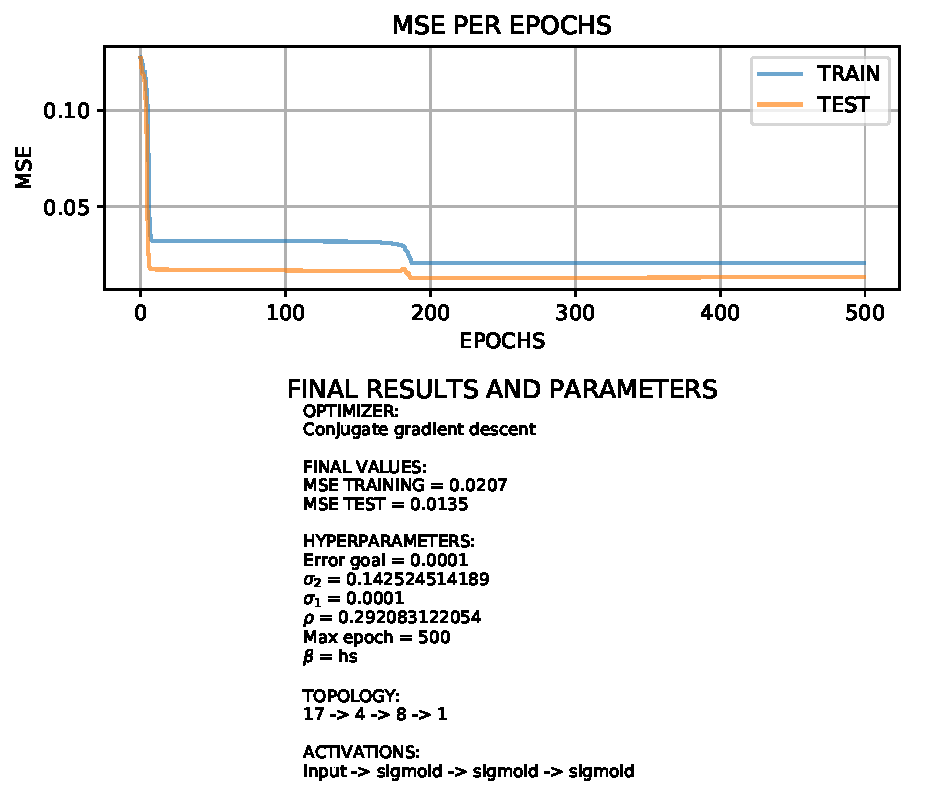
\includegraphics{img/CGD/HS/cgd_mse_test_hs_monks_3.pdf}
                        }
                        \caption{}
                        \label{fig:monks_3_MSE_CGD_HS}
                    \end{subfigure}
                    \begin{subfigure}{0.60\textwidth}
                        \resizebox{\textwidth}{!}{
                            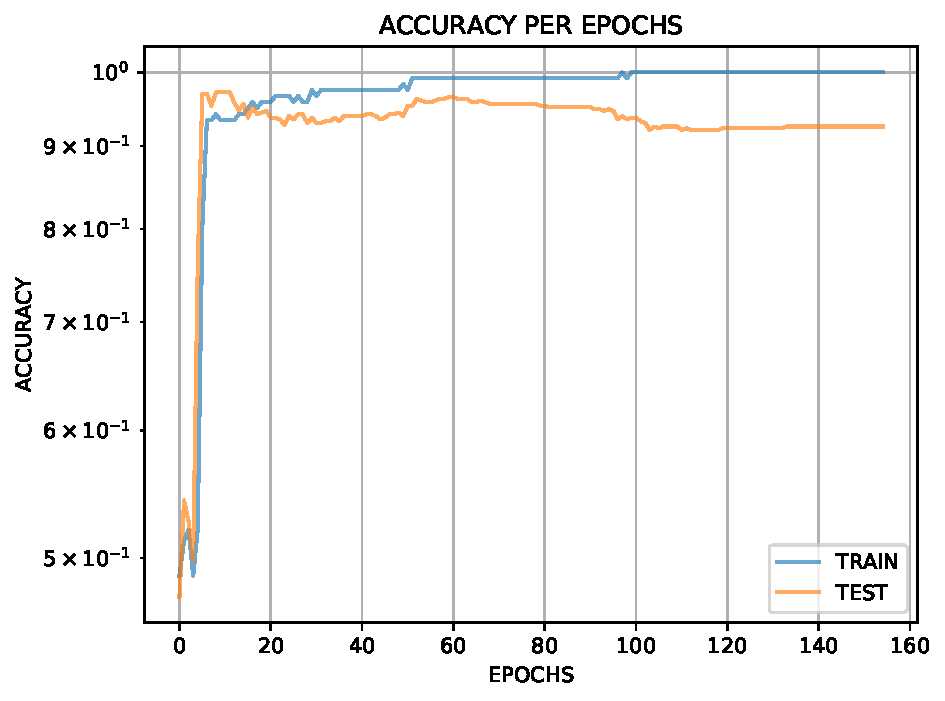
\includegraphics{img/CGD/HS/cgd_accuracy_test_hs_monks_3.pdf}
                        }
                        \caption{}
                        \label{fig:monks_3_ACC_CGD_HS}
                    \end{subfigure}
                    \caption{Example of a final learning curve on MONKS 3.}
                    \label{fig:monks_3_CGD_HS}
                \end{figure}

            % subsection hs (end)

            \subsection{$PR^+$} % (fold)
            \label{sub:pr}

                \begin{figure}[H]
                    \centering
                    \begin{subfigure}{0.60\textwidth}
                        \resizebox{\textwidth}{!}{
                            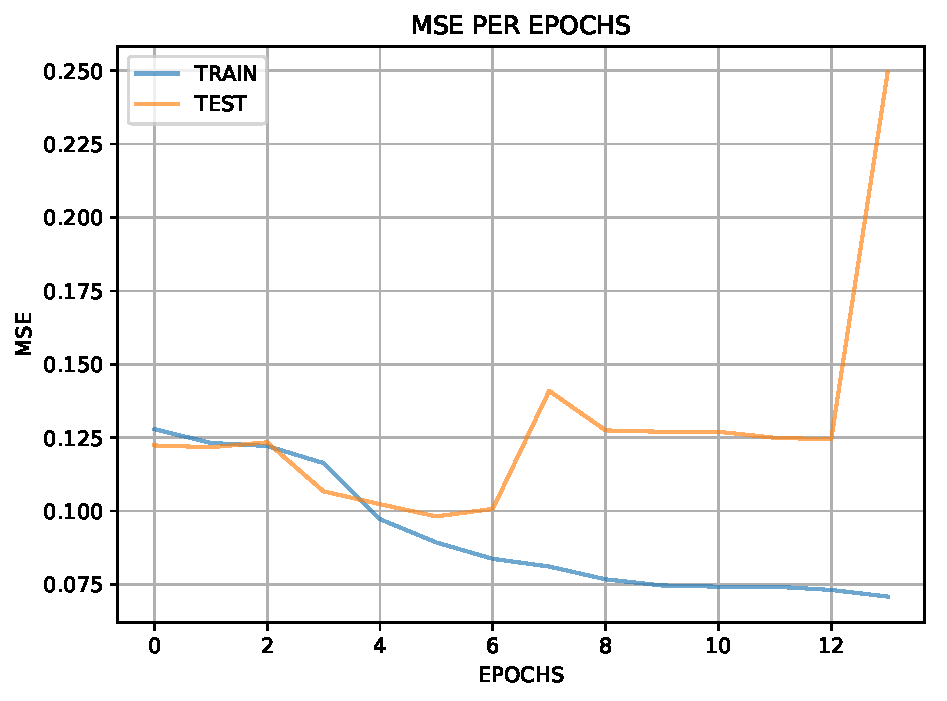
\includegraphics{img/CGD/PR/cgd_mse_test_pr_monks_1.pdf}
                        }
                        \caption{}
                        \label{fig:monks_1_MSE_CGD_PR}
                    \end{subfigure}
                    \begin{subfigure}{0.60\textwidth}
                        \resizebox{\textwidth}{!}{
                            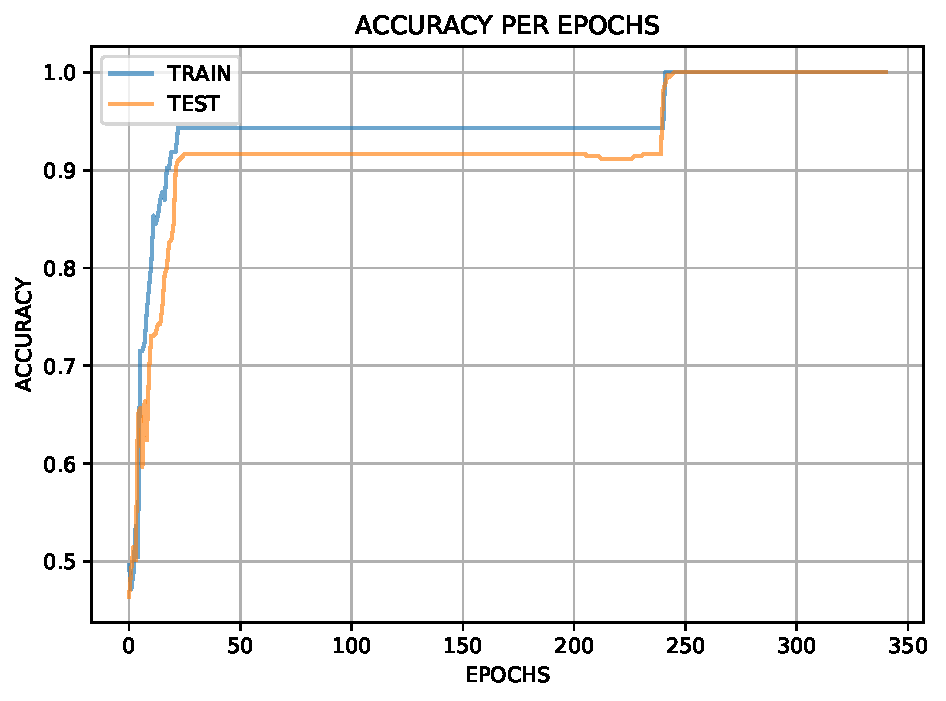
\includegraphics{img/CGD/PR/cgd_accuracy_test_pr_monks_1.pdf}
                        }
                        \caption{}
                        \label{fig:monks_1_ACC_CGD_PR}
                    \end{subfigure}
                    \caption{Example of a final learning curve on MONKS 1.}
                    \label{fig:monks_1_CGD_PR}
                \end{figure}

                \begin{figure}[H]
                    \centering
                    \begin{subfigure}{0.60\textwidth}
                        \resizebox{\textwidth}{!}{
                            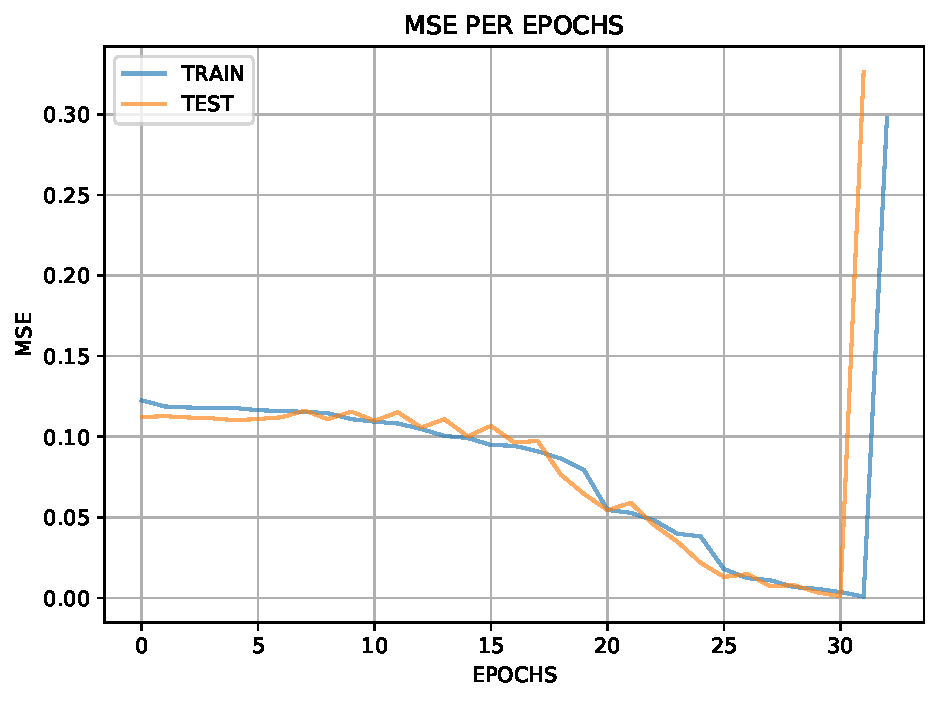
\includegraphics{img/CGD/PR/cgd_mse_test_pr_monks_2.pdf}
                        }
                        \caption{}
                        \label{fig:monks_2_MSE_CGD_PR}
                    \end{subfigure}
                    \begin{subfigure}{0.60\textwidth}
                        \resizebox{\textwidth}{!}{
                            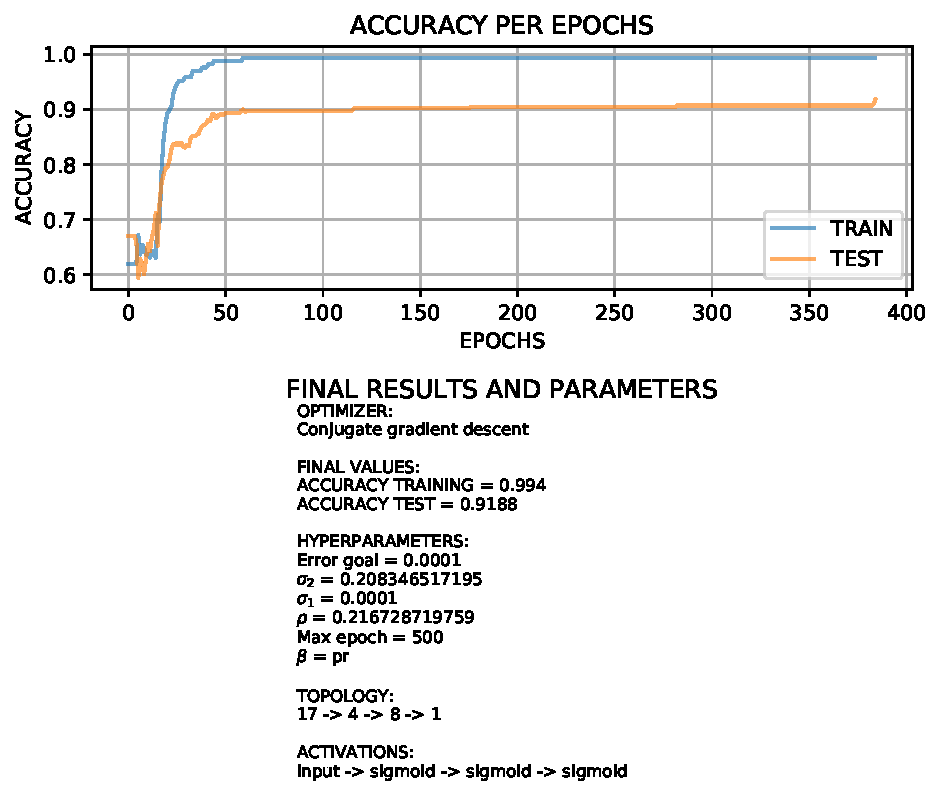
\includegraphics{img/CGD/PR/cgd_accuracy_test_pr_monks_2.pdf}
                        }
                        \caption{}
                        \label{fig:monks_2_ACC_CGD_PR}
                    \end{subfigure}
                    \caption{Example of a final learning curve on MONKS 2.}
                    \label{fig:monks_2_CGD_PR}
                \end{figure}

                \begin{figure}[H]
                    \centering
                    \begin{subfigure}{0.60\textwidth}
                        \resizebox{\textwidth}{!}{
                            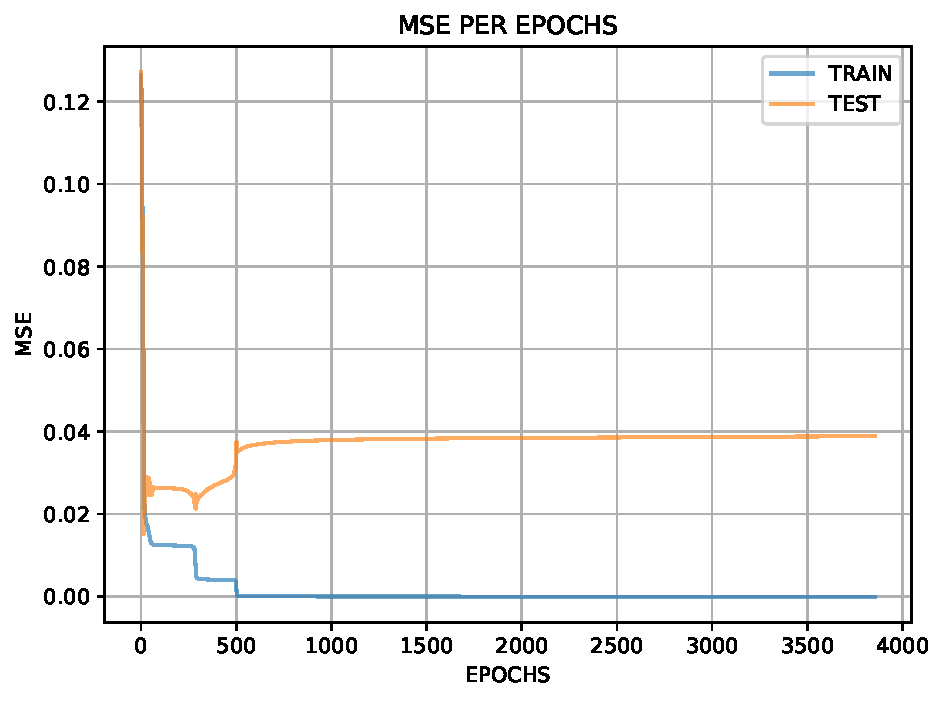
\includegraphics{img/CGD/PR/cgd_mse_test_pr_monks_3.pdf}
                        }
                        \caption{}
                        \label{fig:monks_3_MSE_CGD_PR}
                    \end{subfigure}
                    \begin{subfigure}{0.60\textwidth}
                        \resizebox{\textwidth}{!}{
                            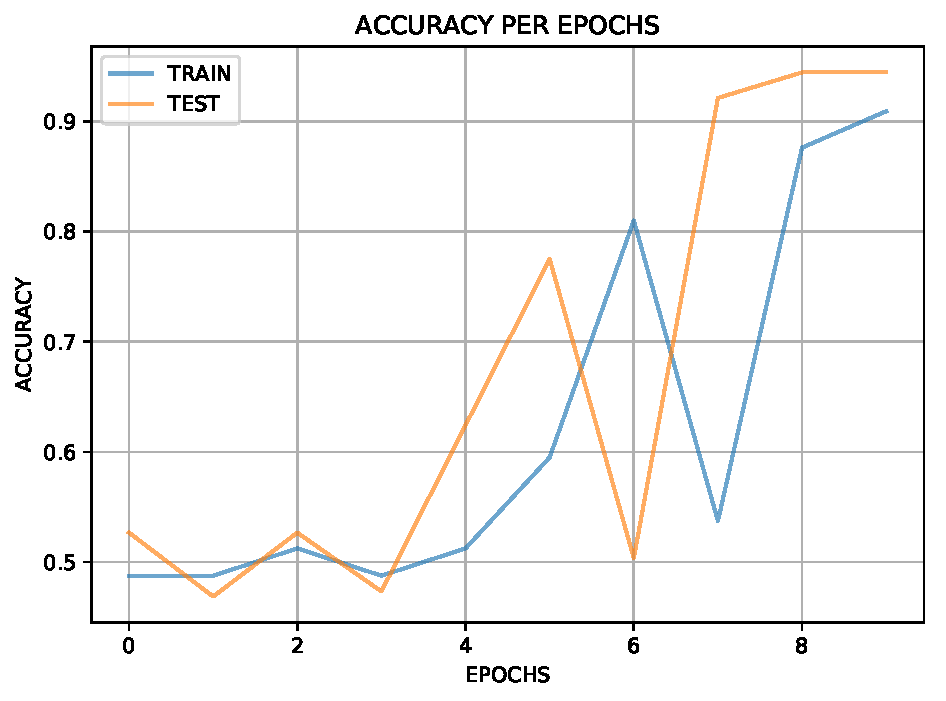
\includegraphics{img/CGD/PR/cgd_accuracy_test_pr_monks_3.pdf}
                        }
                        \caption{}
                        \label{fig:monks_3_ACC_CGD_PR}
                    \end{subfigure}
                    \caption{Example of a final learning curve on MONKS 3.}
                    \label{fig:monks_3_CGD_PR}
                \end{figure}

            % subsection pr (end)

        % section conjugate_gradient_methods (end)

    % chapter monks_learning_curves (end)

    \chapter{CUP's learning curves} % (fold)
    \label{cha:cup_learning_curves}
        As in the previous section, the following curves are the result of the final tests on the test dataset. It has been plotted one of the 10 trails we used for building the statistics we presented in Section \ref{sec:cup}, hence each plot presents a possible learning curve for the best hyperparameters’ selection for each dataset.
        \section{Stochastic Gradient Descent} % (fold)
        \label{sec:cup_sgd}

            \begin{figure}[H]
                \centering
                    \resizebox{\textwidth}{!}{
                        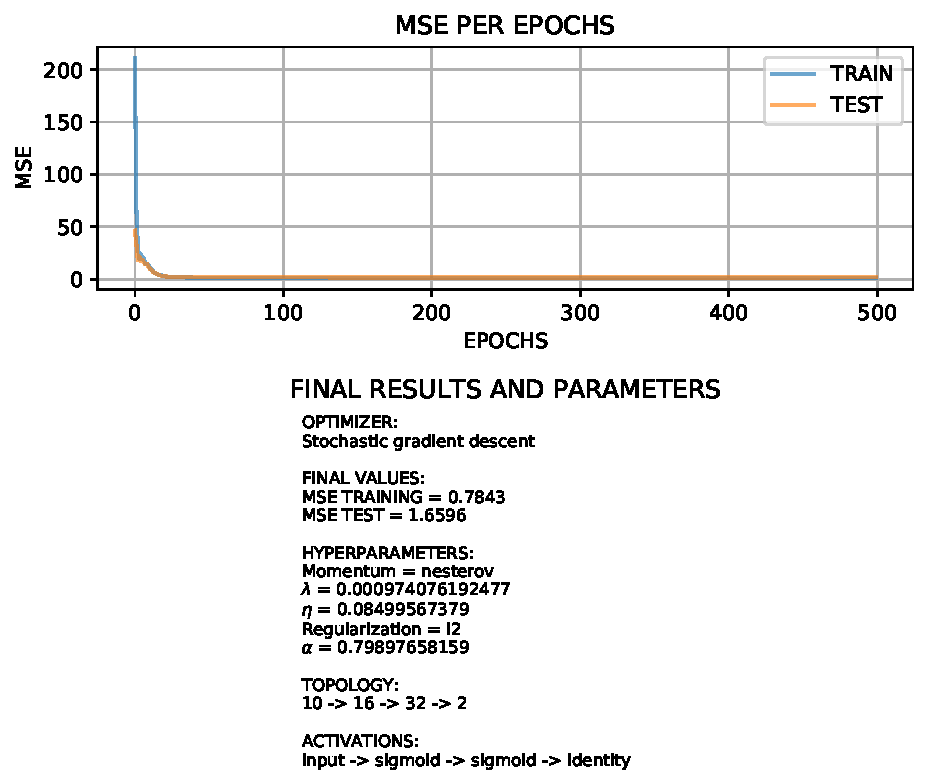
\includegraphics{img/SGD/sgd_mse_test_cup.pdf}
                    }
                    \label{fig:cup_MSE_SGD}
                \caption{Example of a final learning curve on CUP.}
                \label{fig:cup_SGD}
            \end{figure}

        \section{Conjugate Gradient Methods}
        \label{sec:cgd}
            \subsection{$MHS^+$}
            \label{sec:cup_msh}

                \begin{figure}[H]
                    \centering
                        \resizebox{\textwidth}{!}{
                            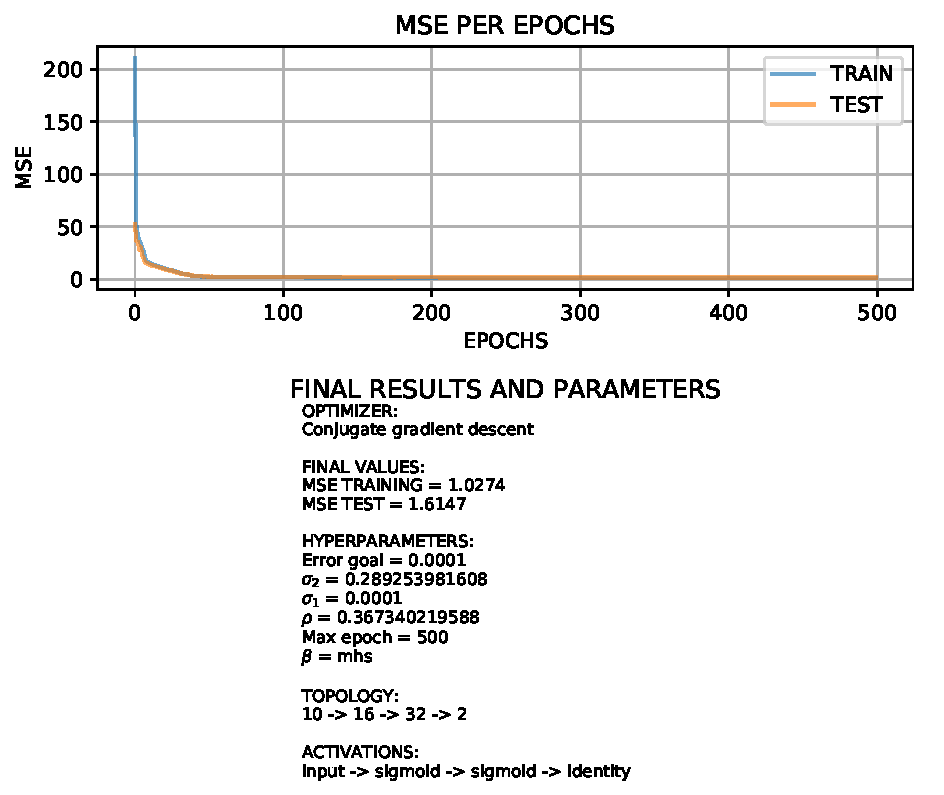
\includegraphics{img/CGD/cgd_mse_test_mhs_cup.pdf}
                        }
                        \label{fig:cup_mhs}
                    \caption{Example of a final learning curve on CUP.}
                \end{figure}

            \subsection{$HS^+$}
            \label{sec:cup_hs}

                \begin{figure}[H]
                    \centering
                        \resizebox{\textwidth}{!}{
                            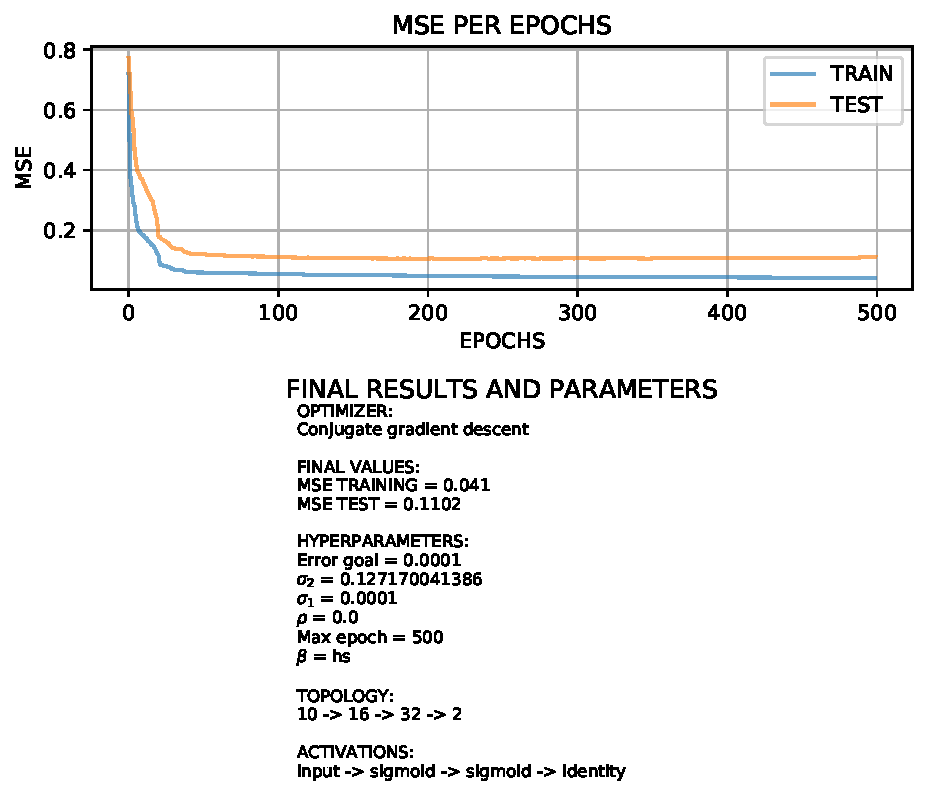
\includegraphics{img/CGD/cgd_mse_test_hs_cup.pdf}
                        }
                        \label{fig:cup_hs}
                    \caption{Example of a final learning curve on CUP.}
                \end{figure}

            \subsection{$PR^+$}
            \label{sec:cup_pr}

                \begin{figure}[H]
                    \centering
                        \resizebox{\textwidth}{!}{
                            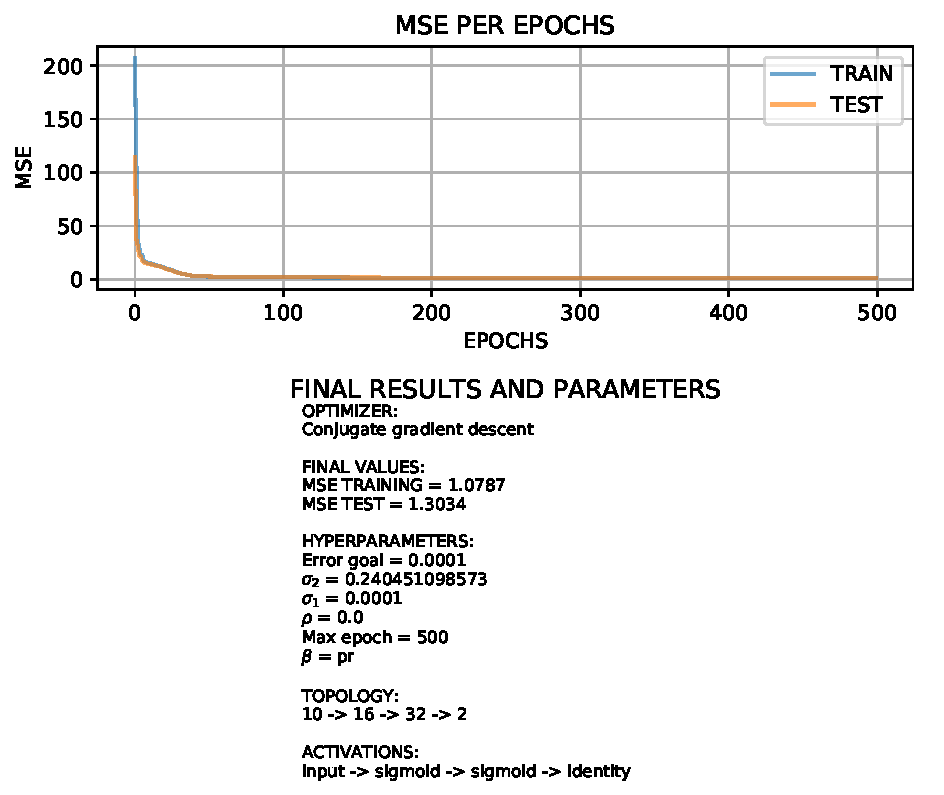
\includegraphics{img/CGD/cgd_mse_test_pr_cup.pdf}
                        }
                        \label{fig:cup_pr}
                    \caption{Example of a final learning curve on CUP.}
                \end{figure}
        % section sgd (end)

\end{appendices}
